\documentclass{beamer}
\usetheme{Boadilla}
\usepackage[utf8]{inputenc}
\usepackage{graphicx}
\usepackage{hyperref}

\title{Análise de Oportunidades de Negócio - Segmento INSS}
\author{Lucas Martin De Lucca}
\date{\today}

\begin{document}

\begin{frame}
  \titlepage
\end{frame}

\begin{frame}{Visão Geral do Projeto}
  \begin{itemize}
    \item Análise de oportunidades de negócio no segmento de beneficiários do INSS para a abertura de agências bancárias.
    \item Utilização de dados públicos de benefícios concedidos de Janeiro a Março de 2025.
    \item Fonte de Dados: Portal de Dados Abertos do Governo Federal.
    \item Total de Registros: 1.565.270 novos benefícios.
  \end{itemize}
\end{frame}

\begin{frame}{Parte 1: As Cidades Mais Atrativas}
  \frametitle{Top 30 Cidades por Volume de Benefícios}
  \begin{figure}
    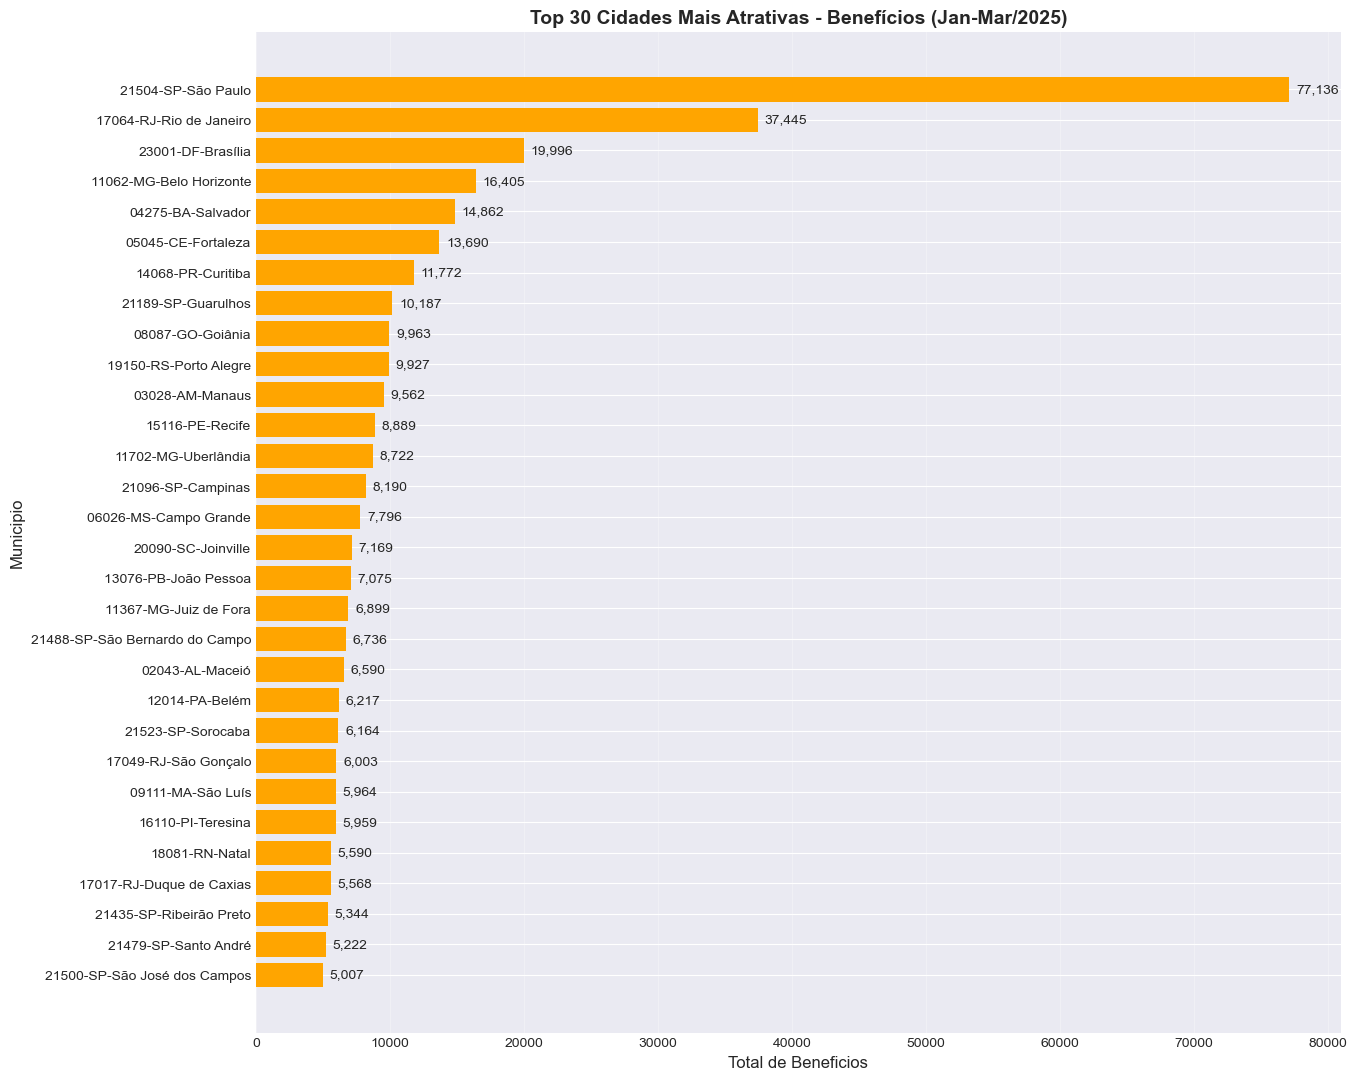
\includegraphics[width=0.9\textwidth]{analise_case_inss_10_0.png}
    \caption{As 30 cidades principais concentram 22,7\% de todos os benefícios concedidos no período.}
  \end{figure}
\end{frame}

\begin{frame}{Parte 2: Análise de Viabilidade Financeira}
  \frametitle{Modelo de Negócio e Ponto de Equilíbrio}
  \begin{columns}
    \begin{column}{0.5\textwidth}
      \textbf{Custos e Receitas:}
      \begin{itemize}
        \item Investimento/agência: R\$ 100.000
        \item Custo Fixo/agência: R\$ 15.000/mês
        \item Custo por Cliente: R\$ 50/mês
        \item Receita por Cliente: R\$ 150/mês
      \end{itemize}
      \vfill
      \textbf{Margem de Contribuição:} R\$ 100/cliente
    \end{column}
    \begin{column}{0.5\textwidth}
      \textbf{Ponto de Equilíbrio Mensal:}
      \begin{itemize}
        \item \textbf{150 clientes} por agência.
      \end{itemize}
      \vfill
      \textbf{Breakeven do Investimento (30 agências):}
      \begin{itemize}
        \item Média de 118.683 novos benefícios/mês.
        \item Com 100\% de conversão, o breakeven ocorre em \textbf{8 dias}.
      \end{itemize}
  \end{column}
  \end{columns}
\end{frame}

\begin{frame}{Parte 2: Análise de Sensibilidade do Breakeven}
  \begin{figure}
    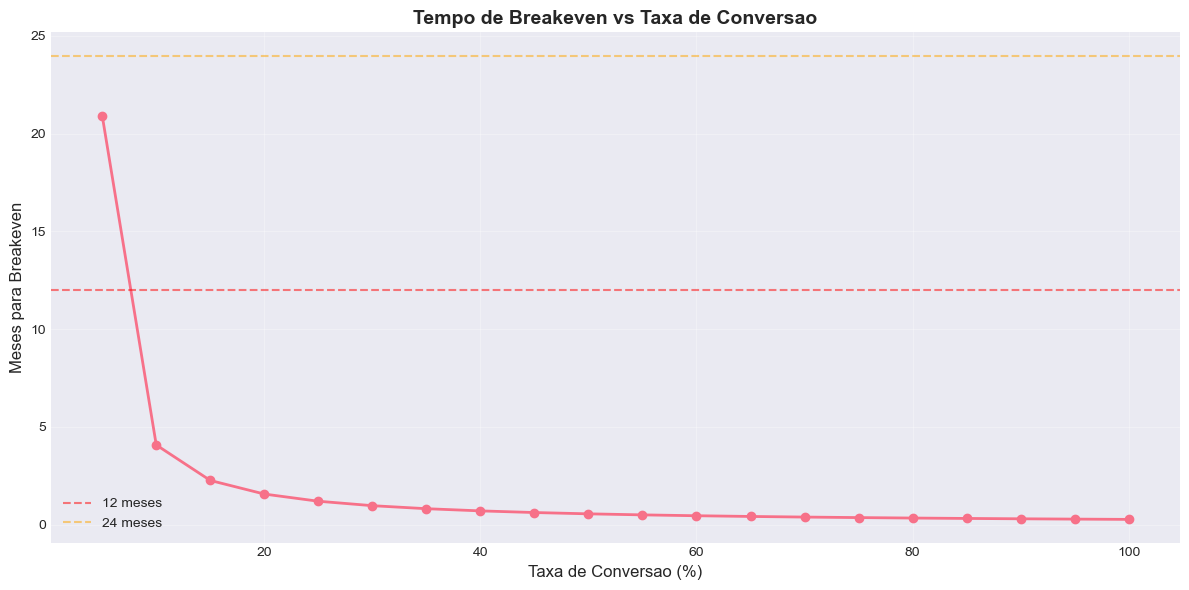
\includegraphics[width=\linewidth]{analise_case_inss_20_0.png}
    \caption{Mesmo com uma taxa de conversão de 10\%, o breakeven é alcançado em apenas 2,5 meses.}
  \end{figure}
\end{frame}


\begin{frame}{Parte 3: Impacto da Duração dos Benefícios}
  \frametitle{Análise de Rotatividade (Churn)}
    \begin{columns}
    \begin{column}{0.5\textwidth}
      \begin{figure}
        \includegraphics[width=\linewidth]{analise_case_inss_24_0.png}
        \caption{Distribuição de Benefícios.}
      \end{figure}
    \end{column}
    \begin{column}{0.5\textwidth}
      \textbf{Principais Pontos:}
      \begin{itemize}
        \item 46,3\% dos benefícios são temporários (auxílios).
        \item A taxa de churn mensal média é de 21.32\%.
        \item Mesmo com a alta rotatividade, o breakeven é atingido no primeiro mês, devido ao alto volume de novos clientes.
      \end{itemize}
    \end{column}
  \end{columns}
\end{frame}

\begin{frame}{Desafio Opcional: Novo Produto de Crédito}
  \frametitle{Potencial de Lucro com Crédito Consignado}
  \begin{itemize}
    \item \textbf{Público-alvo:} Beneficiários permanentes.
    \item \textbf{Premissas:} 20\% de contratação, taxa de juros de 1,6\% a.m., prazo de 30 meses e 5\% de inadimplência.
  \end{itemize}
  \vfill
  \textbf{Resultados Financeiros:}
  \begin{itemize}
    \item \textbf{Receita no 1º Mês (Juros):} R\$ 5,9 milhões
    \item \textbf{Valor Total Emprestado:} R\$ 368 milhões
    \item \textbf{Lucro Líquido em 30 Meses:} \textbf{R\$ 74,9 milhões}
  \end{itemize}
  \vfill
  \textbf{Conclusão:} O crédito consignado representa uma oportunidade de receita e lucro adicional extremamente significativa.
\end{frame}

\begin{frame}{Principais Insights de Negócio}
  \begin{enumerate}
    \item \textbf{Oportunidade Massiva:} Mercado de beneficiários INSS com volume expressivo e constante.
    \item \textbf{Concentração Geográfica:} Foco nas 30 principais cidades otimiza a expansão.
    \item \textbf{Viabilidade Excepcional:} Breakeven em menos de 1 mês, mesmo com alta rotatividade.
    \item \textbf{Modelo Resiliente:} O alto volume de novos clientes supera o churn.
    \item \textbf{Oportunidade de Cross-Sell:} Crédito consignado com potencial de lucro de R\$ 75 milhões.
  \end{enumerate}
\end{frame}

\begin{frame}{Recomendações Estratégicas}
  \begin{itemize}
    \item \textbf{Fase 1:} Implementar agências nas Top 10 cidades para capturar 49\% do volume das 30 principais.
    \item \textbf{Fase 2:} Expandir para as demais cidades da lista após validação do modelo.
    \item \textbf{Foco no Cliente:} Priorizar beneficiários permanentes devido ao maior \textit{lifetime value}.
    \item \textbf{Cross-Sell:} Introduzir o produto de crédito consignado após 3-6 meses de operação para maximizar a lucratividade.
  \end{itemize}
\end{frame}

\end{document}
